Triangular centers and vertices of derived triangle produce, we've seen, beautiful loci. But one center, the {\em Mittenpunkt} $X_9$, took us aback. As shown is Figure~\ref{fig:mitten} and on this \href{https://youtu.be/tMrBqfRBYik}{video} \cite[video \#13]{dsr_math_intell_playlist}:

\begin{theorem}
For the 3-periodic family , the Mittenpunkt $X_9$ is stationary at the Billiard's center.
\label{thm:olga}
\end{theorem}

This fact can be proven by an affine transformation \cite{olga19_mitten} explained in Figure~\ref{fig:mitten}. 

\begin{figure}[H]
     \centering
    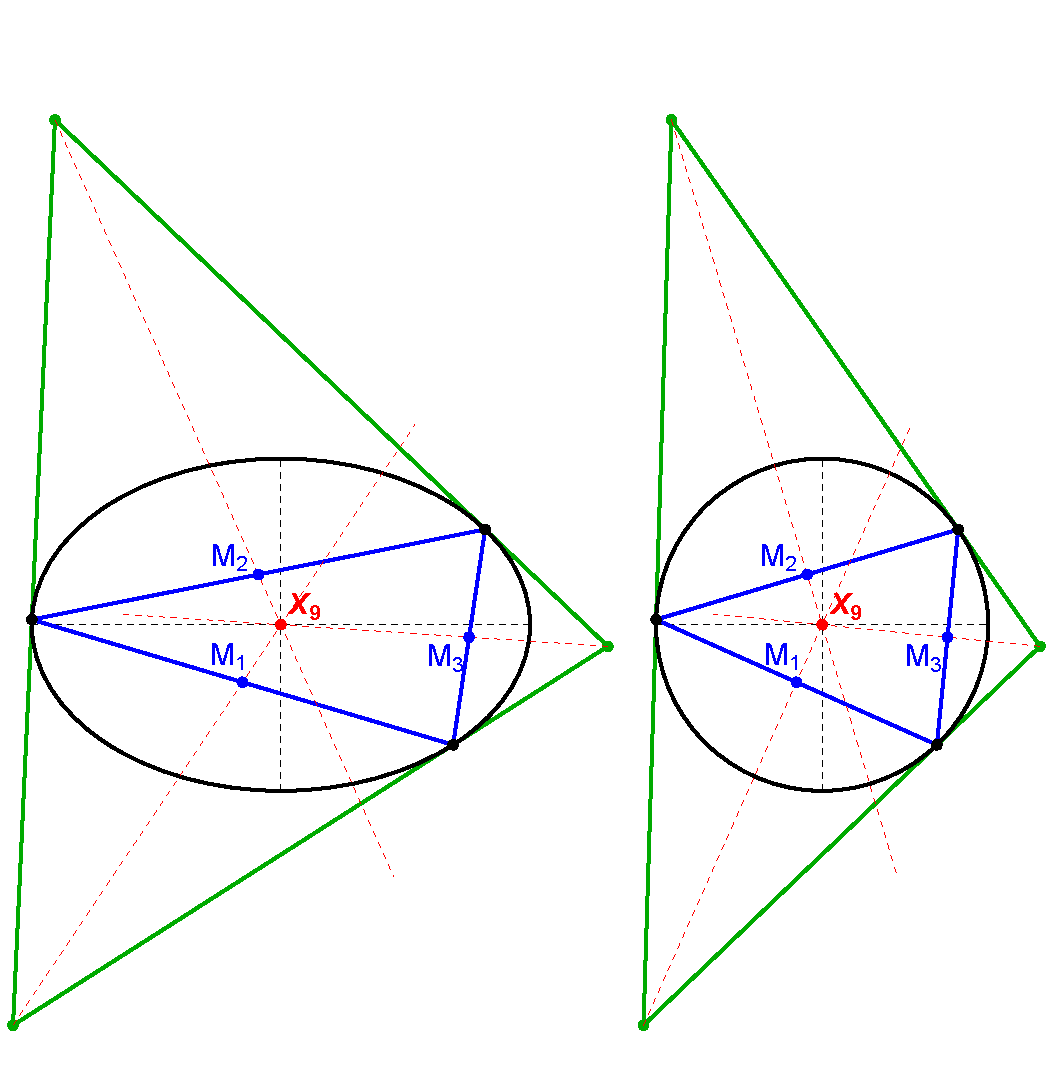
\includegraphics[width=.8\linewidth]{pics/u0051_mitten_proof.pdf}    
     \caption{Affine proof (pun intended!) \cite{olga19_mitten} for the Stationarity of the Mittenpunkt. \textbf{Left}: $N=3$ orbit (blue), its Excentral Triangle (green), and the construction for $X_9$, the Mittenpunkt, stationary at the center of the Billiard (black). \textbf{Right}: Under a suitable affine transform, the Billiard becomes a circle, side midpoints become {\em chord} midpoints (distance ratios are preserved). By symmetry, lines connecting transformed Excenters to the latter must concur at the circle center, uniquely identified under the transform with the Billiard center.
     % done
     \href{https://youtu.be/tMrBqfRBYik}{Video} \cite[pl\#13]{dsr_math_intell_playlist}}
     \label{fig:mitten} 
\end{figure}

A triangle's {\em Circumellipse} \cite{mw} passes through its three vertices. For $N=3$ orbits, we call this object a {\em Circumbilliard}. Since the orbit's Mittenpunkt $X_9$ is congruent with the Billiard's center, we can state (\href{https://youtu.be/vSCnorIJ2X8}{Video} \cite[pl\#14]{dsr_math_intell_playlist}):
%
\begin{corollary}
Every triangle has a circumellipse to which it is a Billiard orbit, whose center coincides with the triangle's Mittenpunkt.
\end{corollary}
